%
% ================ Lexture 7 ================
%
\hl{L7: GNN on Complex Graphs}
\hlorange{\textbf{Heterogeneous graph}}: Graphs have multiple types of nodes and edges. $G=(V,E,R,T)$, where $r_{ij} \in R$ is a relation type, and $t_i \in T$ is a node type.
\hlorange{\textbf{Dynamic graph}}: Graph structure varies with time.
\hlorange{\textbf{Discrete-time dynamic graph (DTDG)}}: Appears in applications with regularly-
sampled data (\eg \hlblue{traffic forecasting}). $[G^{(1)},\dots,G^{(\tau)}]$, where $G^{(t)}=(V^{(t)}, A^{(t)}, X^{(t)})$.
\hlorange{\textbf{Continuous-time dynamic graph (CTDG)}}: $G^t = (V^t, E^t)$, formed via sequentially updating an initial static graph $G^0 = (V^0, E^0)$ according to a set of temporal evolution events $S=\left\{s(t_1),\dots,s(t_n)\right\}$ happened before $t$.
\textcolor{red}{heterogeneity} and \textcolor{red}{temporal dynamics} cannot be captured by classical GNN layers.
\hlorange{\textbf{Heterogeneous network embedding}}: 1) Extract different types of pairs of heterogeneous nodes (\eg \hlblue{(text, image), (text, text)}). 2) Encode each type of node pair using the corresponding weight-sharing module (\eg \hlblue{text by LSTM, image by CNN}). 3) Use a common prediction layer to decode similarity for different relationships.
\hlorange{\textbf{Meta-path}}: A meta-template $\Phi$ in heterogeneous graph $G$ denoted as $(t_1,r_{(1,2)},t_2,\dots,r_{(l-1,l)},t_l)$, where $t_i \in T$ and $r_{i,j} \in R$ are type of the node and the edge (\eg \hlblue{Author-Paper-Author}).
\hlorange{\textbf{$\Phi$-neighbors}}: $N_\Phi(v_i)$ contains nodes that connect with $v_i$ through a meta-path $\Phi$.
\hlorange{\textbf{Heterogeneous Graph Attention Network (HAN)}}:
1) Aggregate information from $\Phi$-neighbors for each $\Phi \in \Psi$ via node-level attention, where $\Psi$ is the set of $P$ meta-path schemes.
% $\alpha^\Phi_{ij}=\frac{exp(\theta(W^T_\Phi\dot[h^\prime_i||h^\prime_j]))}{\sum_{k\in N_\Phi(v_i)} exp(\theta(W^T_\Phi\dot[h^\prime_i||h^\prime_k]))}$
2) Combine the information aggregated from each type of $\Phi$-neighbors through meta-path-level attention (a score for each type) to generate the node representations.
3) Apply the final embedding to supervised tasks and design different loss functions.
\hlorange{\textbf{Heterogeneous Graph Neural Network (HetGNN, Random-walk-based)}}:
1) Sample and select top-$k$ frequent heterogeneous neighbors for each node by Random Walk with Restart (RWR).
2) Extract different types of node contents to generate node content embedding via node heterogeneous contents encoder NN-1.
3) Aggregate embeddings of the sampled heterogeneous neighbors (\ie Type-based neighbor aggregation through NN-2, and Heterogeneous types combination through NN-3).
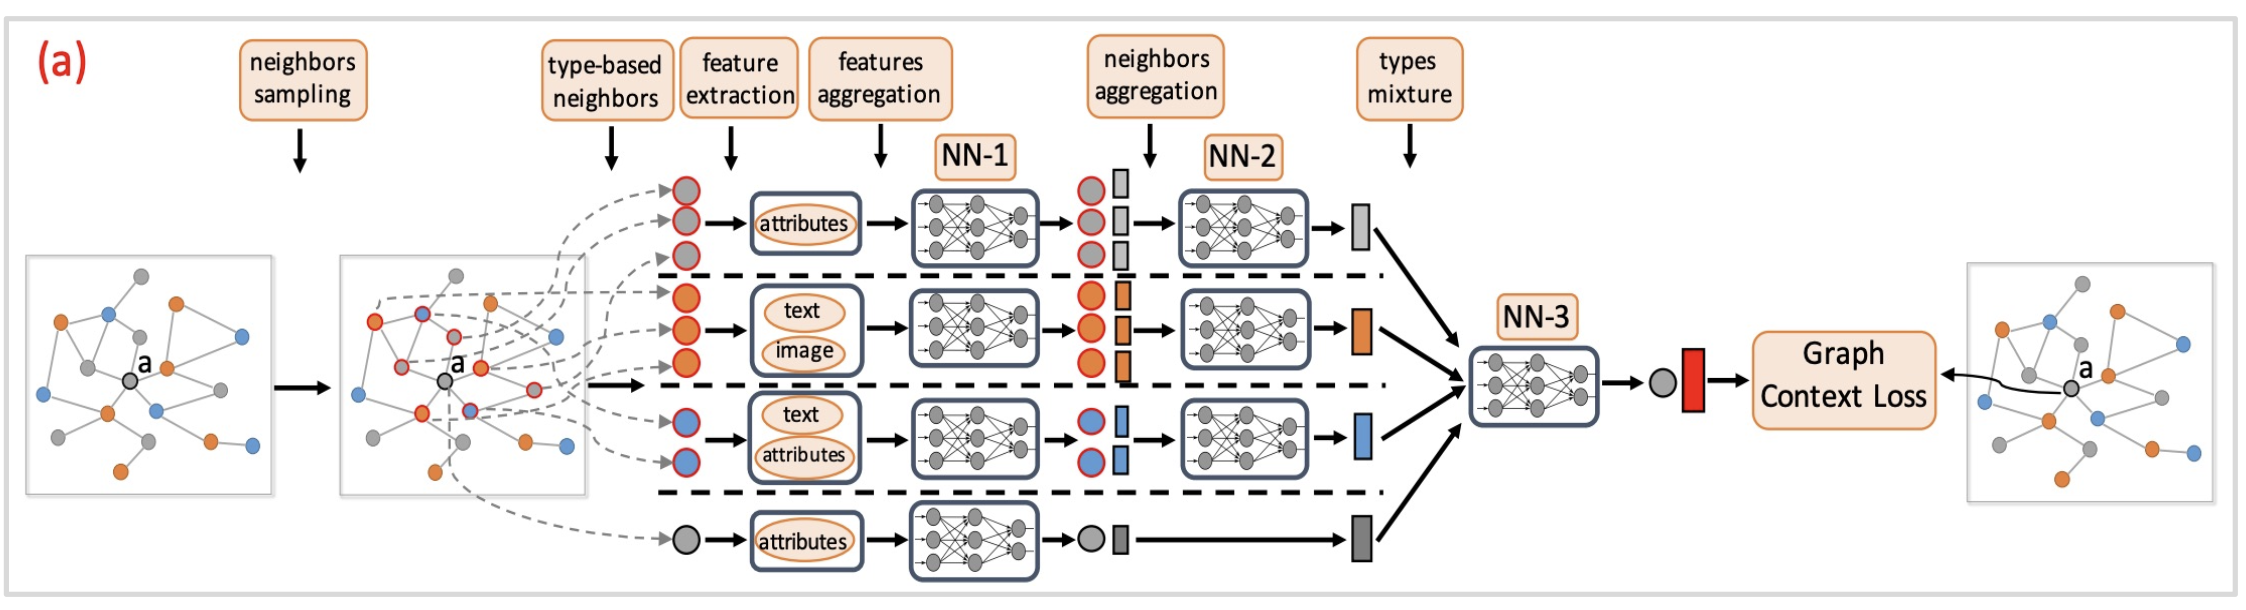
\includegraphics[height=0.052\textwidth]{figs/HetGNN.png}
4) Unsupervised training: Adjacent heterogeneous nodes have similar embeddings. $\mathcal{L}=\sum_{\left \langle v,v_c,v^\prime_c\right \rangle \in T_{walk}} log \sigma(\epsilon_{v_c} \cdot \epsilon_v) + log \sigma (-\epsilon_{v^\prime_c} \cdot \epsilon_v)$, where $\epsilon_v$ is the output embedding, $T_{walk}$ is a set of triplets collected by walk sampling, and $v_c$ is within a distance threshold to $v$ in random walk, and $v^\prime_c$ is a negative node with the same type of $v_c$.
\hlorange{\textbf{Properties of dynamic graphs (DG)}}: 1) Nodes and edges will evolve. 2) Node features and topological structures exhibit temporal patterns.
\hlorange{\textbf{DG evolution types}}: 1) Node and edge addition/deletion. 2) Feature update.
\hlorange{\textbf{DG tasks}}: 1) Extrapolation (\ie predict a future state). 2) interpolation (\ie estimate the past state, like missing value). 3) Time prediction (\ie predict the time for an incoming event).
\hlorange{\textbf{GNN-LSTM for DTDGs}}: 1) Employ a GNN to each graph snapshot $G^t$ and obtain hidden representation $Z^t$. 2) Feed the sequence $[Z^1, \dots,Z^T]$ into LSTM to capture temporal information.
\hlorange{\textbf{EvolveGCN for DTDGs}}: The parameters of GNN at time $t$ are evolved from the model parameters at time $t-1$ by an RNN. $W^{(l-1,t)}=RNN(Z^{(l-1,t)},W^{(l-1,t-1)})$,  $Z^{(l,t)}=GNN(A^{(t)},Z^{(l-1,t)},W^{(l-1,t)})$, where $W^{(l-1,t)}$ are GNN parameters, and $Z^{(l,t)}$ is the GNN output.
\hlorange{\textbf{Joint Dynamic Interaction Embeddings (JODIE) for CTDGs}}: learn dynamic embeddings of each user $u(t)$ and item $i(t)$ at time $t$ from an ordered sequence of temporal user-item interaction events. They use two RNNs to \textcolor{red}{separately} update embeddings of users and items after each interaction. \textcolor{red}{However}, a user’s interests change gradually as time progresses, even without interactions. \textcolor{red}{Therefore}, they predict the future embedding trajectories of users. The model minimizes the $L_2$ distance between the predicted item embedding $\hat{i}(t+\Delta)$ and the real item embedding $i(t^-+\Delta)$ at each interaction. \underline{Limitation}: overlooks the nodes multi-hops away, learns embeddings in a transductive fashion.
\hlorange{\textbf{Temporal Graph Networks (TGN) for CTDGs}}:
1) Memory: stores a state vector $s(t)$ for each node, acting as a condensed representation of all past interactions for each node.
2) Message function: Given an interaction between nodes $i$ and $j$ at time $t$, it two messages ($m_i(t)$ and $m_j(t)$), which are used to update the memory.
3) Memory updater: Aggregate all the messages of node $i$ before time $t$ by an RNN.
4) Graph embedding: Compute the embedding of a node by aggregating the state vector $s(t)$, edge features $e(t)$, and node features $v(t)$ of temporal neighbors. \underline{Staleness problem}: compute embedding of an inactive node by aggregating state vectors of active neighbors.
5) Model training: edge prediction (self-supervised) or node classification (semi-supervised).
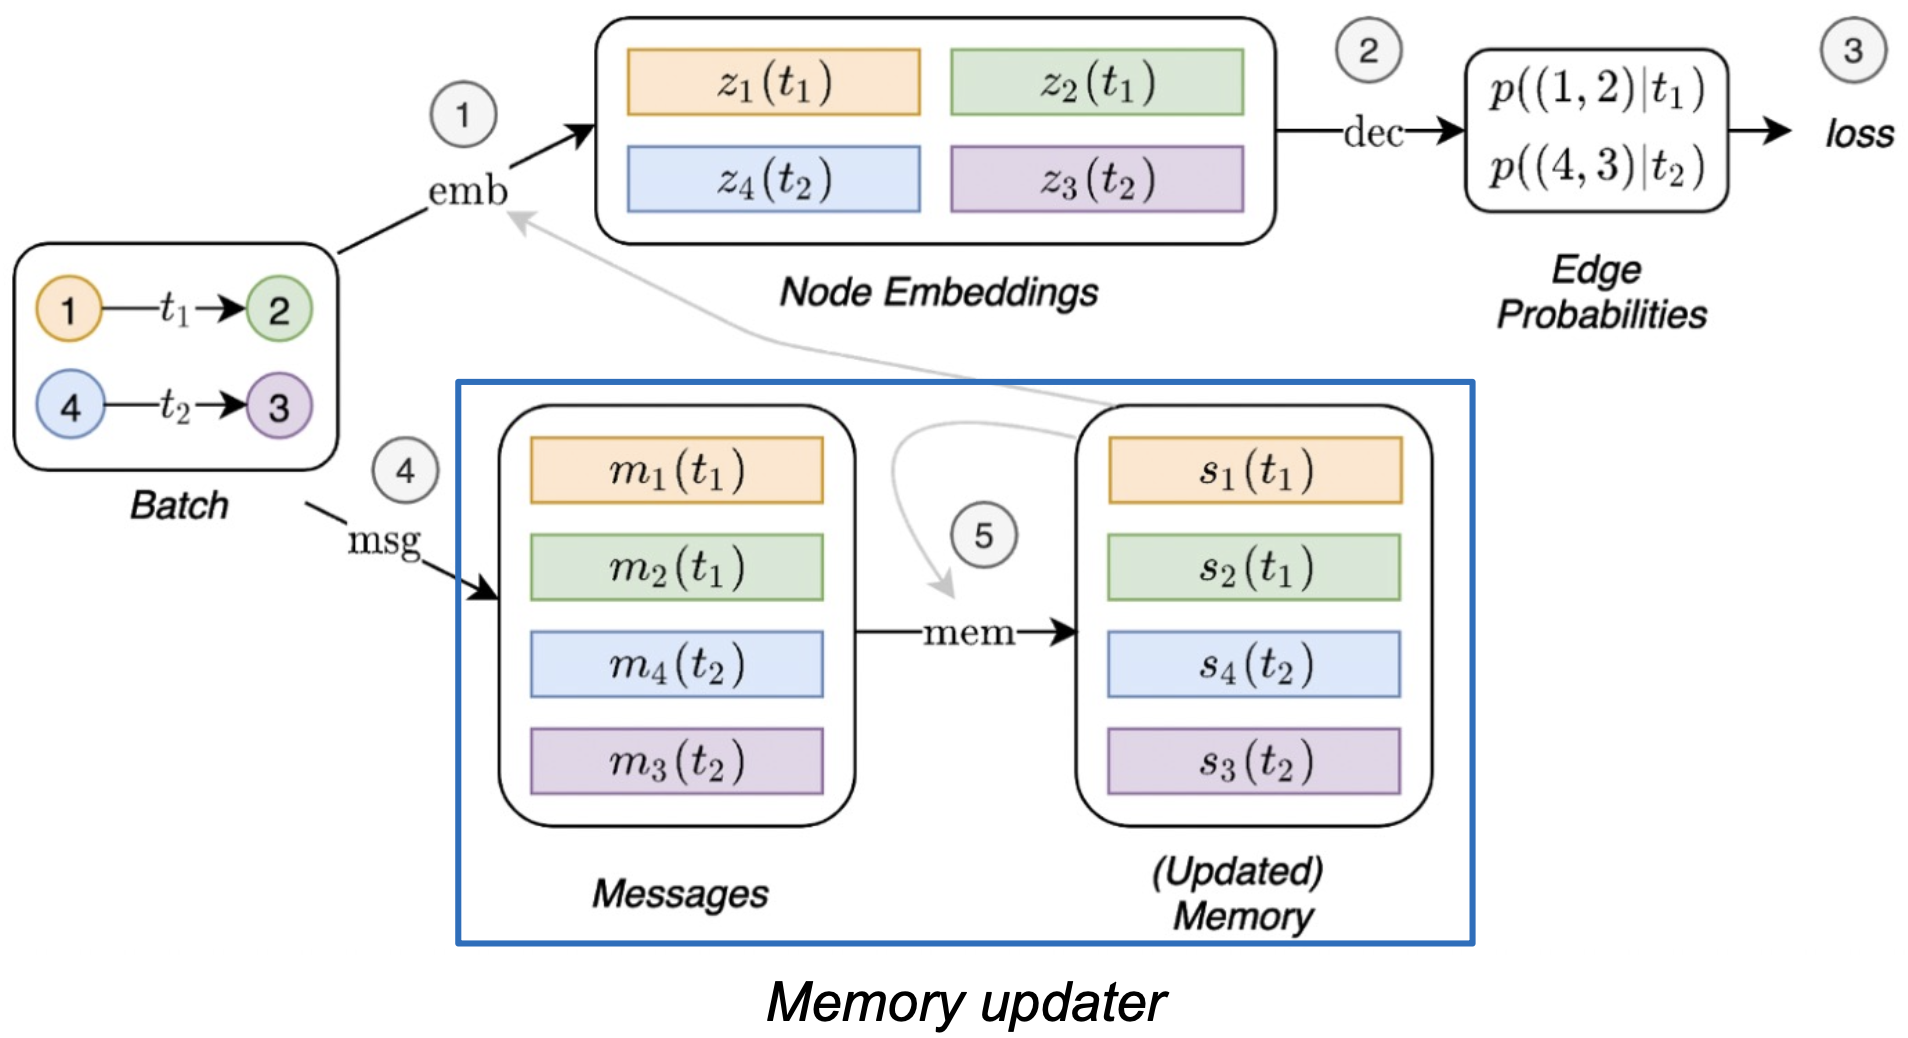
\includegraphics[height=0.07\textwidth]{figs/TGN.png}

%
% ================ Lexture 8 ================
%

\hl{L8: Knowledge Graph}
\hlorange{\textbf{Knowledge Graph (KG)}}: Given a set $\mathcal{E}$ of entities and a set $R$ of relations, a knowledge graph $G$ can be expressed as $G(\mathcal{E}, R, \mathcal{E})$. A triplet  $(h,r,t) \in G$ denotes head entity $h\in \mathcal{E}$ has relation $r \in R$ with tail entity $t\in \mathcal{E}$.
\hlorange{\textbf{KG Applications}}: 1) Link prediction. 2) Triple classification (\ie correct or not). 3) Conversational Recommender Systems.
\hlorange{\textbf{Automatic KG Construction}}:
1) Construct triplets through relationships between entities.
2) Entity and relation embedding: Project entities and relations in the embeddings vector space $R^d$.
3) Representation learning: Given a triple $(h,r,t)$, let $f_r(h,t)=||h+r-t||$ close to 0.
4) Optimization: $\mathcal{L}=\sum_{(h,r,t) \in G}\sum_{(h^\prime,r^\prime,t^\prime) \in G^\prime} (f_r(h,t) - f_r(h^\prime,t^\prime) + \gamma)$, where $\gamma$ is the margin, $G$ are correct triplets, and $G^\prime$ are incorrect ones.
\hlorange{\textbf{KG relation types}}: 1) Symmetric (\eg \hlblue{roommate}). 2) Antisymmetric (\eg \hlblue{teacher}). 3) Inverse (\eg \hlblue{employer and employee}). 4) Composition (\eg \hlblue{My mother's husband is my father}). 5) 1-to-N relations (\eg \hlblue{teacher teaches stu\_1, \dots, stu\_N}).
\hlorange{\textbf{TransE}}: project entities and relations into Euclidean spaces and optimize embeddings by $f_r(h,t)=||h+r-t|| \rightarrow 0$. It \textcolor{red}{can} model 1) Antisymmetric, 2) Inverse, and 3) Composition. But \textcolor{red}{cannot} model 1) Symmetric and 2) 1-N relations.
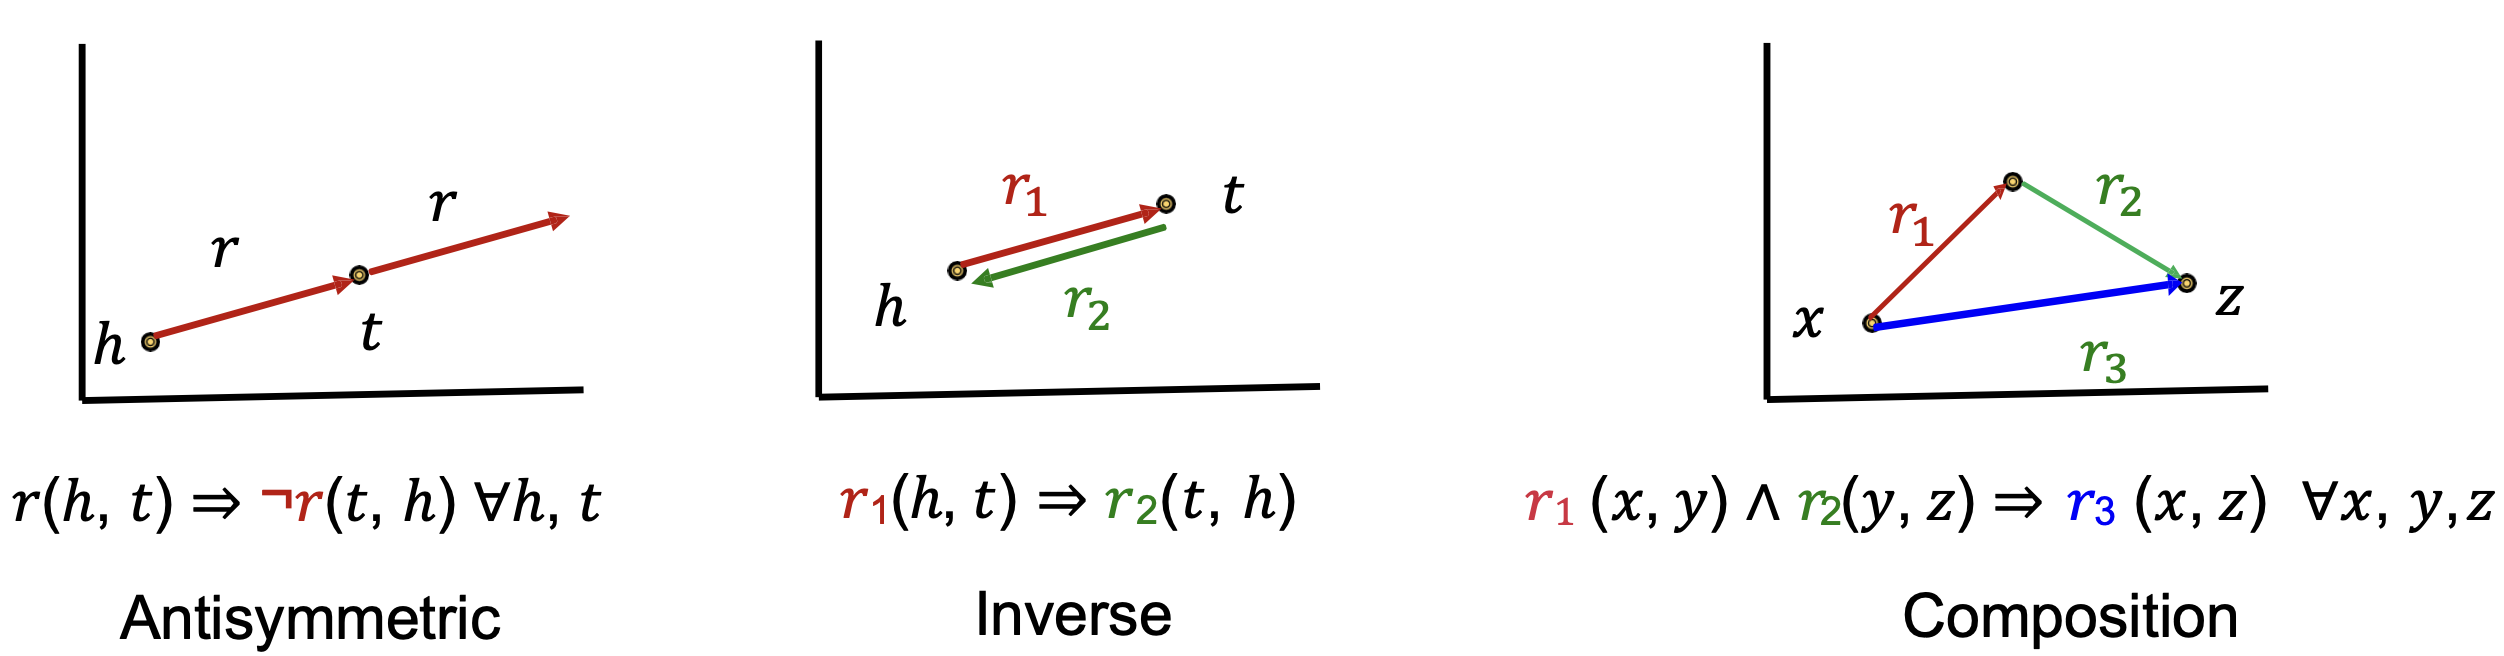
\includegraphics[height=0.05\textwidth]{figs/TransE.png}
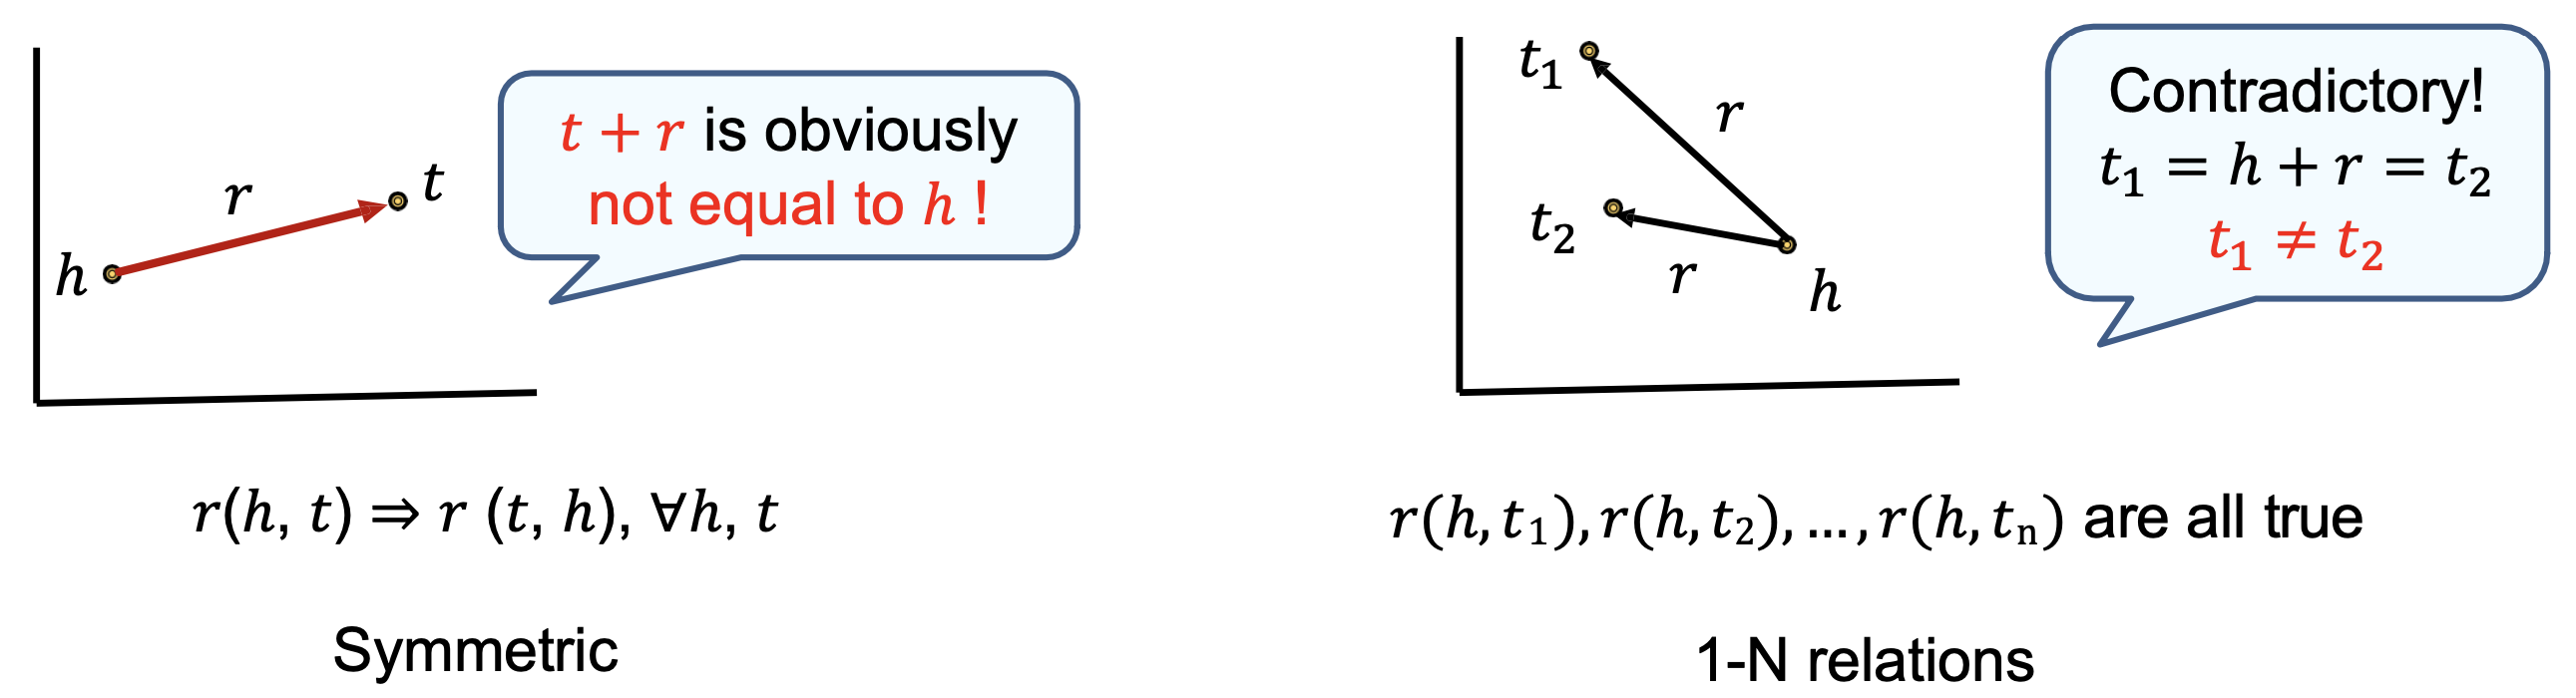
\includegraphics[height=0.05\textwidth]{figs/TransE2.png}
\hlorange{\textbf{TransH}}: Project entity embeddings into relation hyperplanes, TransH \textcolor{red}{can} model 1-N relations. \underline{Project}: $h_\perp=h-W^T_rhW_r$, $t_\perp=t-W^T_rtW_r$, where $W_r$ are learnable parameters. \underline{Score function}: $f_r(h,t)=||h_\perp+r-t_\perp||$.
\hlorange{\textbf{TransR}}: Models entities and relations in entity space and relation spaces, and performs translation in relation space. TransR \textcolor{red}{can} model symmetric and 1-N relations. \underline{Project}: $h_\perp=M_rh$, $t_\perp=M_rt$. \underline{Score function}: $f_r(h,t)=||h_\perp+r-t_\perp||$.
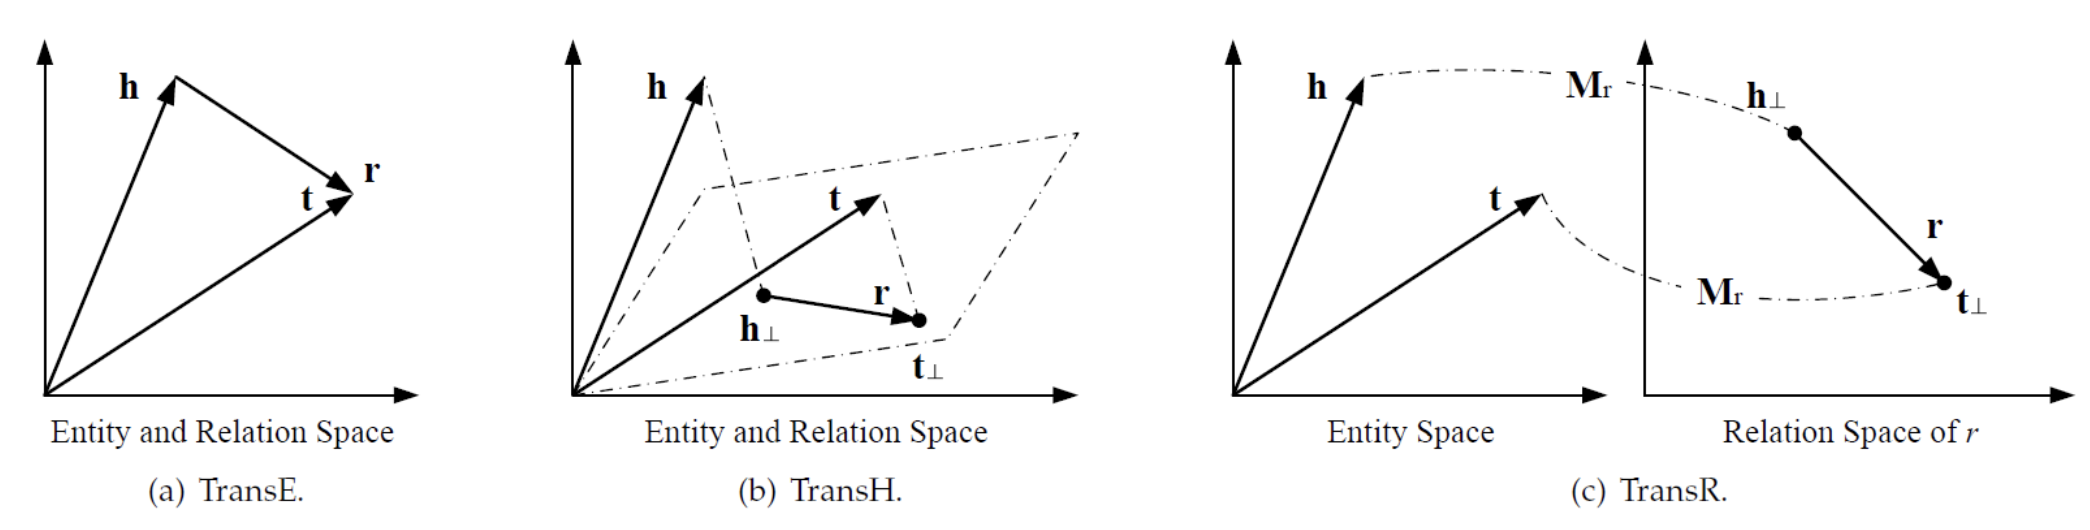
\includegraphics[height=0.05\textwidth]{figs/TransEHR.png}
\hlorange{\textbf{Semantic matching models}}: exploit similarity-based scoring function by neural networks, measuring plausibility of facts by matching \textcolor{red}{latent semantics of entities and relations}.
\hlorange{\textbf{RESCAL}}: \underline{Score function}: $f_r(h,t)=h^T M_r t = \sum^d_i \sum^d_j [h]_i \cdot [M_r]_{ij} \cdot [t]_j$, where $M_r \in R^{d \times d}$ is a matrix associated with the relation.
\hlorange{\textbf{DistMult}}: Simplifies RESCAL by restricting $M_r$ to diagonal matrices. It only captures pairwise interactions between the components of $h$ and $t$ along the \textcolor{red}{same dimension}. \underline{Score functions}: $f_r(h,t)= h^T diag(M_r) t = \sum^d_i [h]_i \cdot [M_r]_i \cdot [t]_i$.
\textcolor{red}{NOTE}: RESCAL and DistMult can only model \textcolor{red}{symmetric} relations.
\hlorange{\textbf{TuckER}}: A KG triplet can be given as a $n\times n \times m$ tensor, where $n$ is number of entities and $m$ is the number of relations. TuckER can decompose the matrix in three directions, obtaining the head entity embeddings, relation embeddings, and tail entity embeddings. \underline{Score function}: $f_r(h,t) = W \times_1 h \times_2 r \times_3 t$, where $\times_n$ indicating the tensor product along the $n^{th}$ mode. TuckER applies logistic sigmoid to each score $f_r(h,t)$ to obtain the predicted probability $p$ of a triplet being true.
\hlorange{\textbf{ConvE}}: 1) Use TransE to get a pre-trained entity and relation embeddings. 2) The entity and relation embeddings are first reshaped and concatenated. 3) The resulting matrix is inputted to a CNN layer. 4) The resulting feature map tensor is projected in a $k$-dimensional space. 5) Calculate the score between $(h, r)$ and $t$ by matching with all candidate tail entity embeddings. \underline{Score function}: $f(vec(f([h,r] * w))W)t$, where $[h,r]$ is the concatenated operation, $w$ is a 2D convolutional filter, and $W$ is a projection matrix.
\hlorange{\textbf{R-GCN}}: Deal with the highly multi-relational data characteristic.
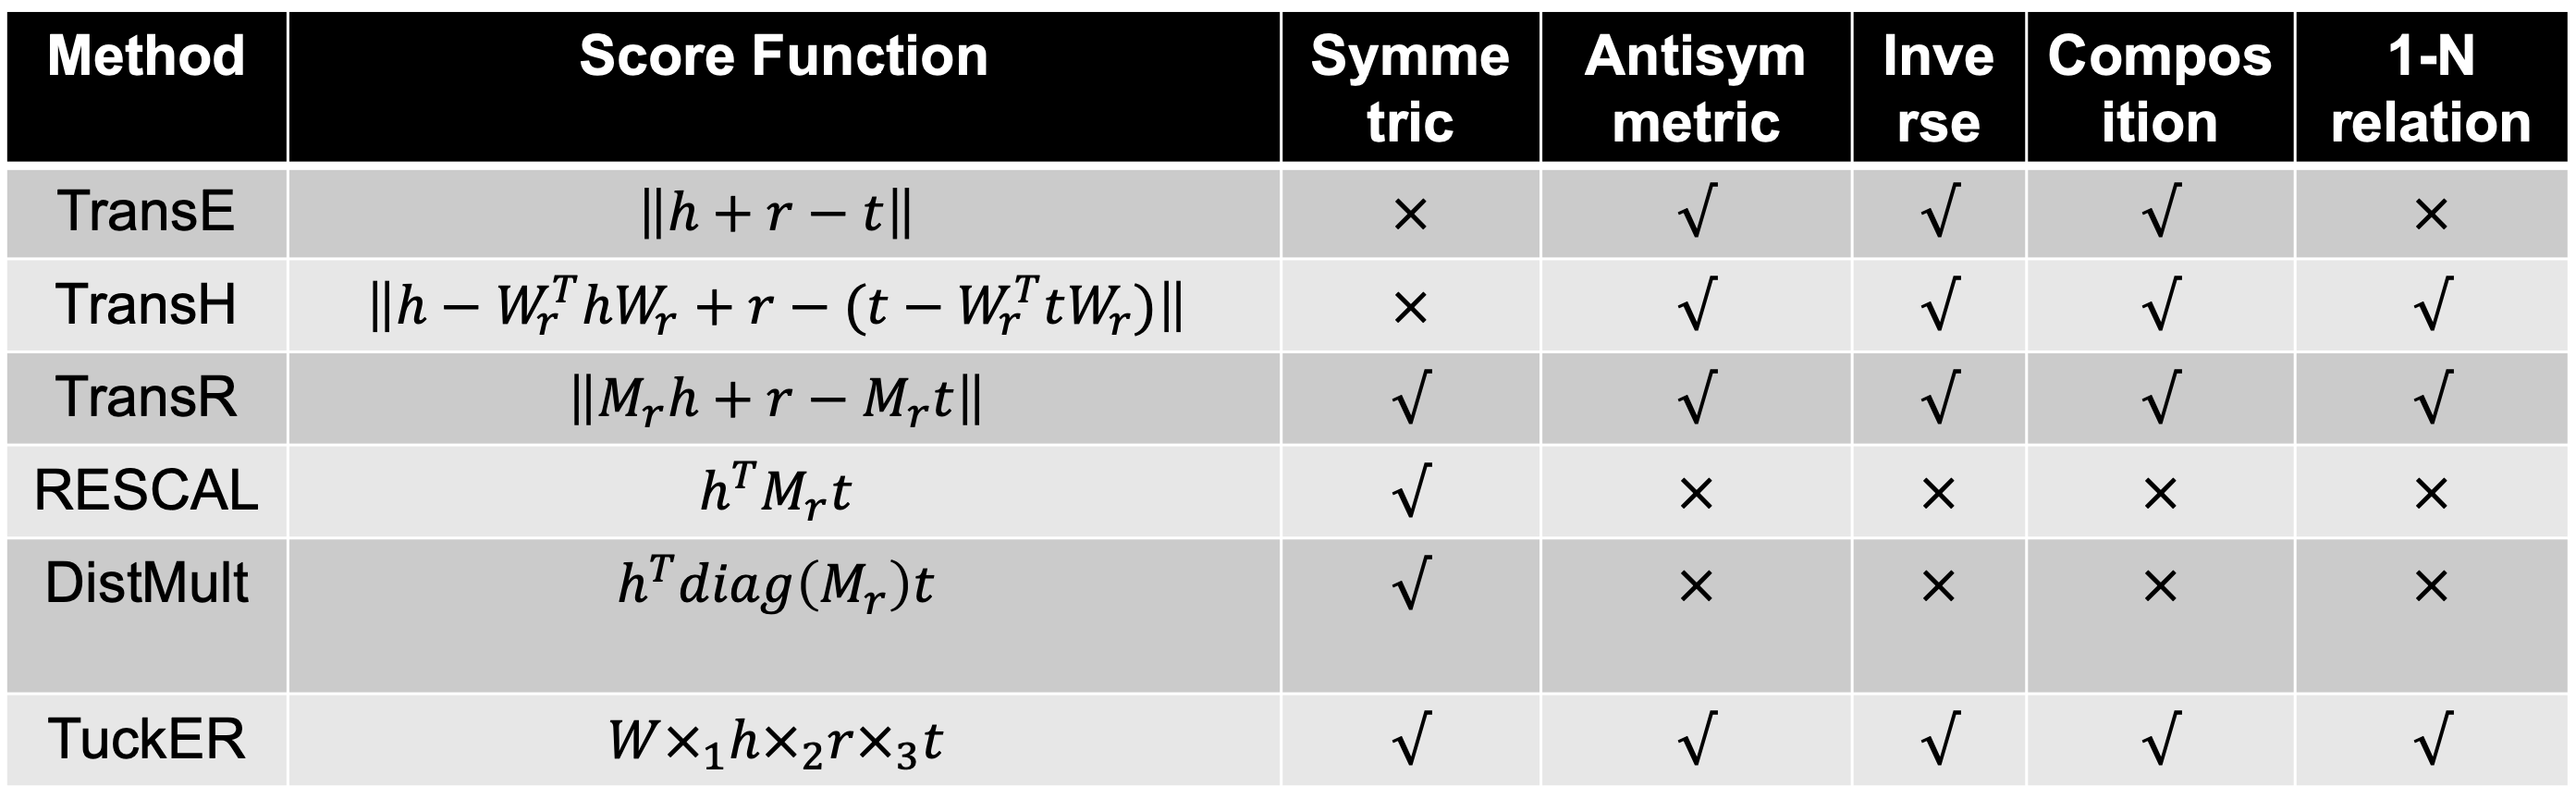
\includegraphics[height=0.06\textwidth]{figs/KGCompare.png}
